\documentclass[a4paper,12pt]{article}
\usepackage[a4paper,top=1.3cm,bottom=2cm,left=1.5cm,right=1.5cm,marginparwidth=0.75cm]{geometry}
\usepackage{cmap}
\usepackage{mathtext}
\usepackage[T2A]{fontenc}
\usepackage[utf8]{inputenc}
\usepackage[english,russian]{babel}
\usepackage{siunitx}
\usepackage{enumitem}
\usepackage{placeins}

\usepackage{graphicx}
\usepackage{subcaption}

\usepackage{wrapfig}
\usepackage{tabularx}
\usepackage{multirow}

\usepackage{hyperref}
\usepackage[rgb]{xcolor}
\hypersetup{
colorlinks=true,urlcolor=blue
}
\usepackage{siunitx}
\usepackage{amsmath,amsfonts,amssymb,amsthm,mathtools}
\usepackage{icomma}
\mathtoolsset{showonlyrefs=false}
\usepackage{euscript}
\usepackage{mathrsfs}
\DeclareMathOperator{\sgn}{\mathop{sgn}}
\newcommand*{\hm}[1]{#1\nobreak\discretionary{}
{\hbox{$\mathsurround=0pt #1$}}{}}

%%% Заголовок
\newcommand\labname{Эффект Поккельса}
\newcommand\labnumber{4.7.2}


\author{Макаров Лев Евгеньевич}
\title{Лабораторная работа №\labnumber

\labname
}

\date{\today}

\begin{document}

\begin{titlepage}
	\begin{center}
		{\large МОСКОВСКИЙ ФИЗИКО-ТЕХНИЧЕСКИЙ ИНСТИТУТ (НАЦИОНАЛЬНЫЙ ИССЛЕДОВАТЕЛЬСКИЙ УНИВЕРСИТЕТ)}
	\end{center}
	\begin{center}
		{\large Физтех-школа фотоники, электроники и молекулярной физики}
	\end{center}
	
	
	\vspace{4.5cm}
	{\huge
		\begin{center}
			{\bf Отчёт о выполнении лабораторной работы \labnumber}\\
			\labname
		\end{center}
	}
	\vspace{2cm}
	\begin{flushright}
		{\LARGE Автор:\\ Макаров Лев Евгеньевич \\
			\vspace{0.2cm}
			Б04-306}
	\end{flushright}
	\vspace{8cm}
	\begin{center}
		Долгопрудный 2025
	\end{center}
\end{titlepage}


\section{Введение}
\textbf{Цель работы:} 
\begin{enumerate}
	\item Исследовать интерференцию рассеянного света, прошедшего кристалл
    \item Наблюдать изменение характера поляризации света при наложении на кристалл электрического поля
\end{enumerate}

\textbf{В работе используются:} гелий-неоновый лазер, поляризатор, кристалл ниобата лития, матовая пластинка, экран, источник высоковольтного переменного и постоянного напряжения, фотодиод, осциллограф, линейка.


\section{Теоретические сведения}
\subsection{Интерференционные кольца при прохождении света через одноосный кристалл}
\begin{figure}[h]
    \center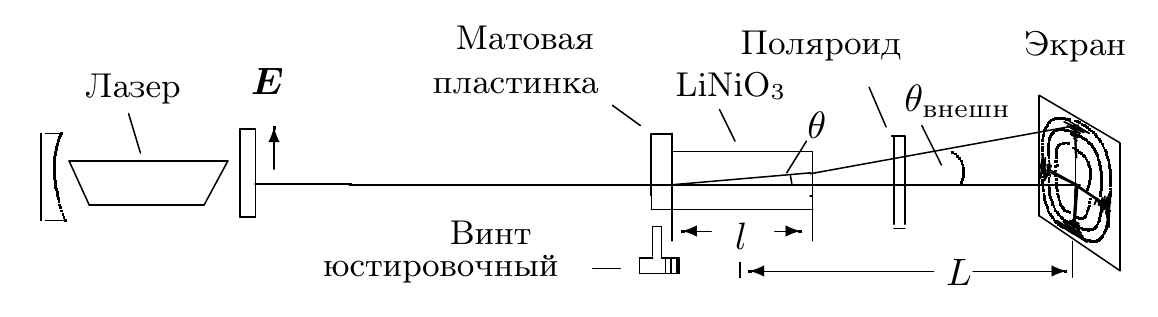
\includegraphics[width = 0.8\linewidth]{pictures/ustanovka_kolca.png}
    \caption{Схема для наблюдения интерференционной картины}\label{fig:ustanovka_kolca}
\end{figure}

При прохождении света через одноосный кристалл, показатель преломления необыкновенной
волны зависит от угла между направлением распространения волны и осью кристалла
по формуле

\begin{equation}
    \frac{1}{n_2^2} = \frac{\cos^2 \theta}{n_o^2} + \frac{\sin^2 \theta}{n_e^2}
    \label{eq:pokazatel_prelomlenia}
\end{equation}

Если считать, что $(n_o - n_e) \ll n_o$, то при малых углах $\theta$ можно
воспользоваться приближенной формулой

\begin{equation}
    n_2 \approx n_o - (n_o - n_e) \theta^2
    \label{eq:pokazatel_prelomlenia_approx}
\end{equation}

Показатель преломления обыкновенного луча не зависит от направления распространения:
$n_1 = n_o$. Если длине кристалла $l$, то после прохождения через кристалл между
обыкновенным и необыкновенным лучом набегает разность фаз

\begin{equation}
    \Delta \varphi = \frac{2\pi}{\lambda} l (n_1 - n_2) \approx
    \frac{2\pi}{\lambda} l (n_o - n_e) \theta^2
    \label{eq:raznost_faz}
\end{equation}

Для случая, когда разрешенное направление анализатора перпендикулярно направлению
поляризации лазера, условием для темного кольца с номером $m$ является
$\varphi = 2\pi m$, откуда следует

\begin{equation}
    \theta_m^2 = \frac{\lambda m}{l(n_o - n_e)}
    \label{eq:theta_m}
\end{equation}

При выхоже из кристалла луч преломляется на границе кристалл-воздух, поэтому угол
$\theta_{внешн} \approx n_o \theta$. Радиус $m$-го темного кольца
$r_m = L\theta_{внешн, m}$. Для квадрата радиуса

\begin{equation}
    r_m^2 = \frac{\lambda}{l} \frac{{(n_o L)}^2}{(n_o - n_e)} m
    \label{eq:r_m}
\end{equation}

\subsection{Эффект Поккельса}

\begin{wrapfigure}{l}{0.4\textwidth}
  \begin{center}
    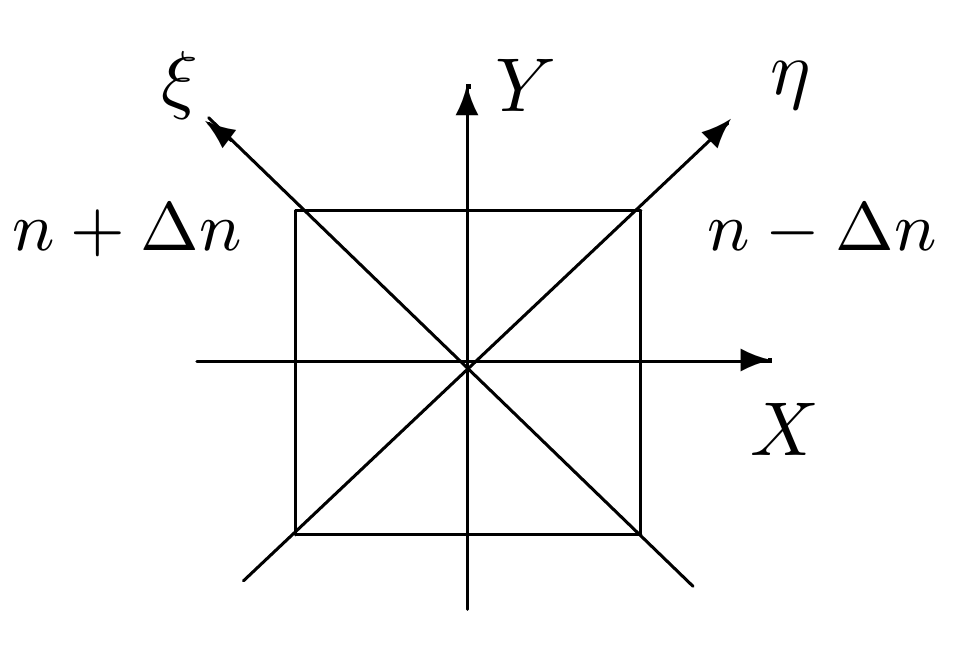
\includegraphics[width=0.38\textwidth]{pictures/pokkels_axes.png}
  \end{center}
  \caption{Главные оси при наличии напряжения вдоль $x$}\label{fig:pokkels_axes}
\end{wrapfigure}

При наличии электрического поля вдоль $x$ в кристалле появляются новые перпендикулярные
главные направления, показатели преломления которых равны $n_o \pm \Delta n$, где
$\Delta n = A \cdot E_{x}$. Пусть поляризация лазера вертикальна, а разрешенное
направление анализатора горизонтальна. Тогда, интенсивность света на выходе
будет зависеть от прикладываемого напряжения ($U = E_x d$) по закону

\begin{equation}
    I = I_0 \sin^2\left(\frac{\pi}{2}\frac{U}{U_{\lambda/2}}\right)
    \label{eq:pokkels}
\end{equation}

где
\begin{equation}
    U_{\lambda/2} = \frac{\lambda}{4A} \frac{d}{l}
    \label{eq:poluvolnovoe_napryajenie}
\end{equation}
\\


\section{Экспериментальная установка}

Оптическая часть установки представлена на рис. \ref{fig:ustanovka_kolca}. Свет гелий-неонового лазера, поляризованный в вертикальной плоскости, проходя сквозь матовую пластинку, рассеивается и падает на двоякопреломляющий кристалл под различными углами. Кристалл ниобата лития с размерами 3 × 3 × 26 мм вырезан вдоль оптической оси Z. На экране, расположенном за скрещенным поляроидом, видна интерференционная картина. Для $\lambda = 0,63 мкм$ (длина волны гелий-неонового лазера) в ниобате лития no = 2,29. Убрав рассеивающую пластинку и подавая на кристалл постоянное напряжение, можно величиной напряжения влиять на поляризацию луча, вышедшего из кристалла. Заменив экран фотодиодом (рис. 3) и подав на кристалл переменное напряжение, можно исследовать поляризацию луча с помощью осциллографа.

\section{Результаты измерений и обработка данных}

\subsection*{I. Юстировка системы}

\begin{enumerate}
    \item Соберем оптическую систему согласно рис. \ref{fig:ustanovka_kolca}. Включим лазер и установим анализатор так, чтобы через него не проходило лазерное излучение.
\end{enumerate}

Узнаем поляризацию при разрешенном направлении, посмотрев через анализатор на отраженный свет под углом Брюстера. Тогда В нашем случае параллельная поляризация.

\begin{enumerate}[resume]
    \item Поставим кристалл и установим перед ним вплотную матовую пластинку. Расстояние от кристалла до экрана $L = 81$ см. 
    \item Получим на экране интерференционную картину. Отцентрируем ее. Повернем анализатор на $90^\circ$ и проверим, что интерференционная картина изменилась на негативную. Вернем анализатор в прежнее положение.
\end{enumerate}

\subsection*{II. Измерения}

\begin{enumerate}[resume]
    \item Измерим радиусы темных колец и построим график зависимости $r^2_m = f(m)$. Результаты измерений запишем в таблицу \ref{table:1}.
\end{enumerate}

\begin{table}[!ht]
    \centering
    \caption{Измерение диаметров колец зеленой пары Ртутной лампы}
    \begin{tabular}{|l|l|l|l|l|l|}
        \hline
        $m$     & 1   & 2   & 3    & 4   & 5 \\ \hline
        $r$, см & 1.5 & 3.5 & 4.75 & 5.5 & 6 \\ \hline
    \end{tabular}
    \label{table:1}
\end{table}

График изобразим на рис. \ref{graph:1}.


\FloatBarrier
\begin{figure}[!h]
    \centering
    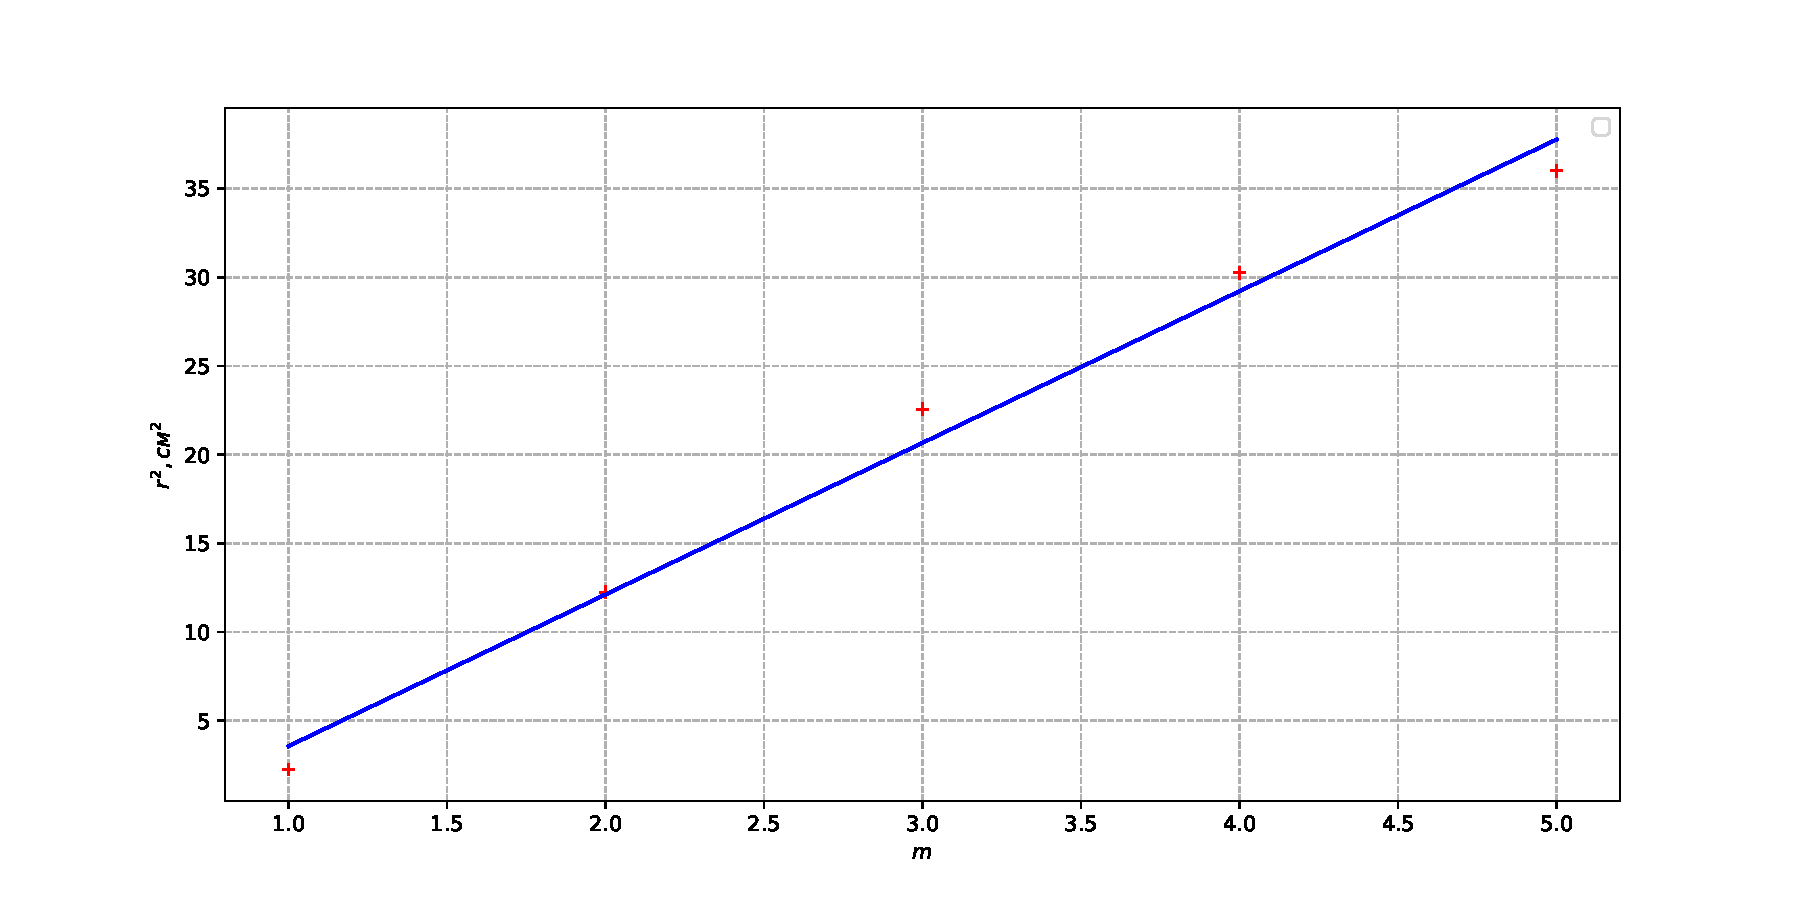
\includegraphics[scale=0.65]{graph-1.pdf}
    \caption{График зависимости $r^2 = f(m)$}
    \label{graph:1}
\end{figure}
\FloatBarrier

\begin{equation*}
    k = (8.55 \pm 0.02) \ \ \text{см}^2
\end{equation*}

из формулы \eqref{eq:r_m}:

\begin{equation*}
    k = \frac{\lambda n_o^2 L^2}{l \left(n_o - n_e\right)} \implies n_e = n_o - \frac{\lambda n_o^2 L^2}{kl} \approx 2.19
\end{equation*}

\begin{enumerate}[resume]
    \item Уберем матовую пластинку, убедимся в центровке системы. 
\end{enumerate}

Подключим разъем блока питания на постоянное напряжение и установим регулятор на минимум.

Определим напряжение $U_{\lambda/2}$, при котором достигается максимум интенсивности.

\begin{equation*}
    U_{\lambda/2} = 300 \ \ \text{В}
\end{equation*}

При $U_{\lambda} = 2U_{\lambda/2}$ достигается минимум.

\begin{enumerate}[resume]
    \item Подадим на кристалл напряжение $U_{\lambda/4} = \frac{1}{2} U_{\lambda/2}$.
\end{enumerate}

На выходе получаем круговую поляризацию. Убедимся в этом, вращая анализатор. Интенсивность при этом практически не меняется, что значит поляризация является эллиптической.

\newpage
\begin{enumerate}[resume]
    \item Установим вместо экрана фотодиод и подключим его к Y-выходу осциллографа. Убрав напряжение до нуля, переключим генератор на переменное напряжение.
    \item Постепенно повышая напряжение пронаблюдаем как меняются фигуры Лиссажу. Определим по ним напряжение $U_{\lambda/2}$, соответствующее переходу от максимума к минимуму.
\end{enumerate}

\begin{equation*}
    U_{\lambda/2} \approx 5 \ \ \text{дел} = 300 \ \ \text{В}
\end{equation*}

\begin{enumerate}[resume]
    \item Зарисуем фигуры Лиссажу для напряжений $U_{\lambda/2}, U_{\lambda/4}, U_{\lambda}$. Изобразим их на рис. \ref{fig:lissazhu}
\end{enumerate}

\begin{figure}[h!]
    \centering
    \begin{subcaptionbox}{Фигура для $U_{\lambda/4}$\label{fig:img1}}[0.3\textwidth]
        {\includegraphics[width=\linewidth]{pictures/lissazhu_1_over_4.png}}
    \end{subcaptionbox}
    \hfill
    \begin{subcaptionbox}{Фигура для $U_{\lambda/2}$\label{fig:img2}}[0.3\textwidth]
        {\includegraphics[width=\linewidth]{pictures/lissazhu_1_over_2.png}}
    \end{subcaptionbox}
    \hfill
    \begin{subcaptionbox}{Фигура для $U_{\lambda}$\label{fig:img3}}[0.3\textwidth]
        {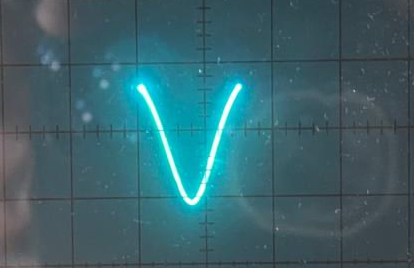
\includegraphics[width=\linewidth]{pictures/lissazhu_1.png}}
    \end{subcaptionbox}
    \caption{\textit{Фигуры Лиссажу}}
    \label{fig:lissazhu}
\end{figure}

\section{Выводы}

В ходе работы была исследована интерференция для рассеянного света, прошедшего через кристалл. Получено двулучепреломление кристалла. 

Получены значение напряжений $U_{\lambda/2}, U_{\lambda/4}, U_{\lambda}$ и фигуры Лиссажу для них.


\end{document}